\renewcommand{\prevlecture}{0 }
\renewcommand{\thislecture}{1 }
\renewcommand{\nextlecture}{2 }

%
% Cover page
%

\title[PHYS 201 / Lecture \thislecture]
{
  PHYS 201 / Lecture \thislecture \\
  {\it Electric charge; Coulomb's law; Superposition principle; Electric field}\\
}

\author[C.Andreopoulos] {
  Professor Costas Andreopoulos\inst{1,2}, {\it FHEA}
}
\institute[Liverpool/STFC-RAL] {
   \inst{1} University of Liverpool, Department of Physics\\
   \vspace{0.1cm}
   \inst{2} U.K. Research \& Innovation (UKRI), Science \& Technology Facilities Council,\\
            Rutherford Appleton Laboratory, Particle Physics Department\\
   \vspace{0.5cm}
   {\it {\color{magenta} Lectures delivered at the University of Liverpool, 2020-21}}\\
   \vspace{0.2cm}
}
\date{\today}

\titlegraphic{
  
\includegraphics[height=25px]{./images/logo/liverpool.png}
  \hspace{3px}
  
\includegraphics[height=30px]{./images/logo/ral.png}
}


\begin{frame}[plain]
  \titlepage
\end{frame}


% ------------------------------------------------------------------------------
% ------------------------------------------------------------------------------

%
%
%

\begin{frame}{Plan for Lecture \thislecture}

\begin{itemize}
{\small
\item {\bf Electric charge}
  \begin{itemize}
  {\scriptsize
    \item The source of electric phenomena
  }
  \end{itemize}

\item {\bf Coulomb's law}
  \begin{itemize}
  {\scriptsize
     \item Describes the force between two point charges
  }
  \end{itemize}

\item {\bf Superposition principle}
  \begin{itemize}
  {\scriptsize
     \item Allows the calculation of the force on a charge from an array of other charges
  }
  \end{itemize}

\item {\bf Continuous distributions of charge}
  \begin{itemize}
  {\scriptsize
    \item Make the leap from discrete to continuous charge distributions described by a charge density
    \item Reformulate Coulomb's law for continuous charge distributions
  }
  \end{itemize}

\item {\bf Electric field}
  \begin{itemize}
  {\scriptsize
     \item This new concept will provide a more fundamental way to think about electric forces
           in terms of a field that permeates space. We will think of ways to visualise it.
  }
  \end{itemize}

}
\end{itemize}

\end{frame}

% ------------------------------------------------------------------------------
% ------------------------------------------------------------------------------

%
%
%

\begin{frame}{Electric charge}

\begin{center}
    The electric charge is an {\bf intrinsic property of matter}
\end{center}

\begin{itemize}
  \item It comes in {\bf two varieties}
    \begin{itemize}
      \item There are positive electric charges and negative electric charges
      \item The electric charge is an algebraic quantity
        \begin{itemize}
           \item A positive charge and an equal negative charge amounts to no charge.
%                Our body contains a large number of positive and negative charges, but it is neutral.
        \end{itemize}
    \end{itemize}
  \item It is {\bf quantised}
    \begin{itemize}
      \item Free charges are multiples of the electron charge
    \end{itemize}
  \item It is {\bf conserved}
    \begin{itemize}
      \item The charge is \underline{conserved globally}
        \begin{itemize}
           \item i.e. the total charge of the universe is fixed for all time
        \end{itemize}
      \item But a stronger statement can also be made: It is \underline{conserved locally}
        \begin{itemize}
            \item i.e. charge can not disappear from here and re-appear in another corner of the world,
                  which would still conserve the charge globally
        \end{itemize}
    \end{itemize}
\end{itemize}

\end{frame}


%
% Quiz
%

{
\problemslide

\begin{frame}{Quiz}

\begin{blockexmplque}{Question}
  What is wrong with the following radioactive decay?
  \begin{equation*}
    \;^{238}_{92}U \rightarrow \;^{234}_{90}Th + \;^{4}_{3}Li
  \end{equation*}

\end{blockexmplque}

\begin{blockexmplans}{Answer}
\noindent
\scalebox{1}[-1]{
%\reflectbox{
 \rotatebox[origin=c]{180}{
   \noindent
   \begin{minipage}[t]{\linewidth}
     Count the numbers of protons on each side!
   \end{minipage}%
 }
}
\end{blockexmplans}


\begin{blockexmplque}{Question}
  Electrons and positrons are produced by the nuclear transformations of
  protons and neutrons known as $\beta$ decay. If a neutron transforms
  into a proton, is an electron or a positron produced?

\end{blockexmplque}

\begin{blockexmplans}{Answer}
\noindent
\scalebox{1}[-1]{
%\reflectbox{
 \rotatebox[origin=c]{180}{
   \noindent
   \begin{minipage}[t]{\linewidth}
     n $\rightarrow$ p + e$^{-}$ + $\bar{\nu}_{e}$
   \end{minipage}%
 }
}
\end{blockexmplans}



\end{frame}

} % ending quiz


%
%
%

\begin{frame}{Electric charge}

In SI, the electric charge unit is measured in {\bf Coulomb (C)}.\\
\vspace{0.1cm}

\begin{itemize}
{\small
\item
The absolute value of the charge of an electron is about 1.6$\times 10^{-19}$ C.
%Therefore, one Coulomb is the charge carried by about 6.24$\times 10^{+18}$ such particles.\\
\item
The amount of charge that travels through an alkaline AA battery till it is fully discharged is about 5000 C.
\item
Electrostatic shocks are caused by charges of few $\mu$C ($10^{-6}$ C)
}
\end{itemize}

\vspace{0.3cm}

In SI, the Coulomb is a {\em derived} unit.\\
\vspace{0.3cm}
One Coulomb is\\
\vspace{0.1cm}
\begin{itemize}
{\small
\item
   the charge carried by a current of one Ampere flowing for one second, or
\item
   the charge on a capacitor of one Farad held to a potential of one Volt.
}
\end{itemize}

\vspace{0.1cm}

Of course, we don't know about Amperes, Farads and Volts just yet.\\
For now, just remember that the electric charge unit is the Coulomb (C).

\end{frame}

%
%
%

\begin{frame}{Point charges}

Later in this lecture we will talk about {\em extended} charge distributions.\\
\vspace{0.2cm}

However, initially (and throughout the course) we will also be talking about {\em point} charges.\\
\vspace{0.2cm}
\begin{itemize}
\item
  A point charge is... well, exactly that. An amount of charge concentrated in a single geometrical point.
\item
  Obviously, this is an approximation.
\item
  However, this is a good approximation when the distances involved in a problem under investigation
  are far larger than the actual "size" of the charges.
\end{itemize}

\end{frame}


% starting reminder
{
\reminderslide

%
%
%

\begin{frame}{Reminder: Scalars and Vectors}

\begin{itemize}

\item {\bf Scalars}
  \begin{itemize}
     \item They are quantities that {\bf have magnitude but no direction}
  \end{itemize}

\vspace{0.3cm}

\item {\bf Vectors}
  \begin{itemize}
     \item They are quantities that {\bf have both magnitude and direction}
     \vspace{0.2cm}
     \item Note that vectors have magnitude and direction {\bf but no location}
     \begin{itemize}
         \item a displaced vector has the same magnitude and direction
     \end{itemize}
  \end{itemize}

\end{itemize}

\vspace{0.3cm}

\begin{center}
  Can you give a few examples of scalar and vector quantities?
\end{center}

\end{frame}


%
%
%

\begin{frame}{Reminder: Vectors}

{\small
Let me draw a {\em right-handed} coordinate system in a 3-D {\em Euclidian} space (below).\\
}
\begin{columns}
  \begin{column}{0.30\textwidth}
   \begin{center}
     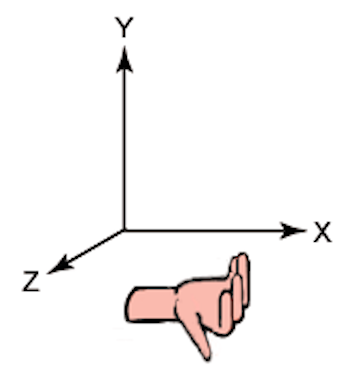
\includegraphics[width=0.90\textwidth]{./images/schematics/right_handed_coordinate_system_1.png}\\
     \vspace{0.3cm}
     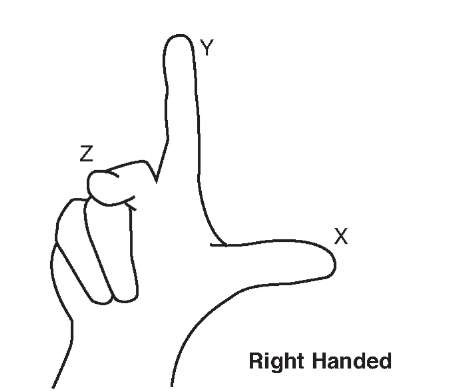
\includegraphics[width=0.90\textwidth]{./images/schematics/right_hand_rule_xyz.png}\\
   \end{center}
  \end{column}
  \begin{column}{0.70\textwidth}
  {\scriptsize
     Explaining "Euclidian":
     \begin{itemize}
     {\scriptsize
      \item
         The term refers to the {\em mathematical structure} of the space: i.e. the relationships
         describing the distance and angles between a set of points, the symmetries (rotations, reflections) of the space etc.
       \item
         From Greek mathematician Euclid of Alexandria, c. 300 BC.
       \item
         The term does not specify the dimensionality (indeed, a Euclidian space can be 1-D, 2-D, 3-D, ...)
       \item
         Not all spaces are Euclidian: Non-Euclidian spaces (e.g. curved spaces) also exist and used in modern physics.
       \item
         {\bf The physical space (as the canvas for usual empirical phenomena) is Euclidian}.
     }
     \end{itemize}
     \vspace{0.4cm}
     {\tiny
      The coordinate system is called {\bf right}-handed for a reason!
      See on left and {\bf take notice}.\\
      If you are right-handed, can't be bothered to leave the pencil from your right hand
      and, instead, you use your other hand to determine the directions
      (as I have seen several students do) then you are in trouble!
      (Unless you have two right hands.)\\
     }
  }
  \end{column}
\end{columns}

\end{frame}

%
%
%

\begin{frame}[t]{Reminder: Vectors}

{\small
 Now, let's draw a {\bf vector $\vec{A}$} in our coordinate system. \\
 \vspace{0.1cm}
 Since vectors have magnitude and direction
 but no location, let's shift it, for convenience, so that it starts at the origin of our coordinate system.
}
\vspace{0.1cm}

\begin{columns}[t]
  \begin{column}{0.45\textwidth}
   \begin{center}
     {\scriptsize
       Let $A_x$, $A_y$, $A_z$ be the components of $\vec{A}$
       along the x,y and z axis respectively.\\
     }
     \vspace{0.3cm}
     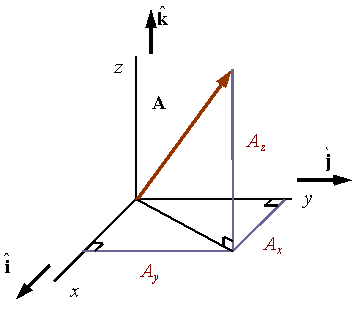
\includegraphics[width=0.98\textwidth]{./images/schematics/vector_in_3D_right_handed_coordinate_system_1.png}\\
     \vspace{0.3cm}
   \end{center}
  \end{column}
  \begin{column}{0.55\textwidth}
  {\scriptsize
     We usually write $\vec{A}$ in terms of its components as:
     \begin{equation*}
       \vec{A} = \Big( A_x, A_y, A_z \Big)
     \end{equation*}
     or
     \begin{equation*}
       \vec{A} = A_x \hat{i} + A_y \hat{j} + A_z \hat{k}
     \end{equation*}
     where $\hat{i}$, $\hat{j}$, $\hat{k}$
     (also usually denoted as  $\hat{x}$, $\hat{y}$, $\hat{z}$)
     are unit vectors along the x, y and z axis respectively:
     $\hat{i}$=(1,0,0), $\hat{j}$=(0,1,0), $\hat{k}$=(0,0,1).\\
     \vspace{0.3cm}
     We can also write $\vec{A} = |\vec{A}| \cdot \hat{A}$
     where $|\vec{A}|$ is the magnitude of $\vec{A}$ ($|\vec{A}|=\sqrt{A_x^2 + A_y^2 + A_z^2}$)
     and $\hat{A}$ is a unit vector ($|\hat{A}|=1$) along $\vec{A}$.\\
  }
  \end{column}
\end{columns}

\end{frame}

%
%
%

\begin{frame}{Reminder: Vector addition and subtraction}

\begin{columns}
  \begin{column}{0.30\textwidth}
   \begin{center}
     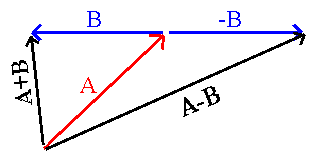
\includegraphics[width=0.98\textwidth]{./images/schematics/vector_addition_and_subtraction_1.png}\\
   \end{center}
  \end{column}
  \begin{column}{0.70\textwidth}
     Let $\vec{A} = \Big( A_x, A_y, A_z \Big)$ and $\vec{B} = \Big( B_x, B_y, B_z \Big)$.\\
  \end{column}
\end{columns}

\vspace{0.3cm}

Then
\begin{equation*}
    \vec{A} + \vec{B} =
    \Big( A_x, A_y, A_z \Big) + \Big( B_x, B_y, B_z \Big) =
    \Big( A_x + B_x, A_y + B_y, A_z + B_z \Big)
\end{equation*}
and
\begin{equation*}
    \vec{A} - \vec{B} =
    \Big( A_x, A_y, A_z \Big) - \Big( B_x, B_y, B_z \Big) =
    \Big( A_x - B_x, A_y - B_y, A_z - B_z \Big)
\end{equation*}

\end{frame}

%
%
%

\begin{frame}{Reminder: Vector multiplication}

We have 3 kinds of multiplication involving vectors:\\
\vspace{0.4cm}
\begin{itemize}
  \item Product {\color{magenta} $\lambda \vec{A}$} of a vector $\vec{A}$ with a scalar $\lambda$\\
        \vspace{0.2cm}
  \item {\bf Dot product} {\color{magenta} $\vec{A} \cdot \vec{B}$} of two vectors $\vec{A}$, $\vec{B}$\\
        \vspace{0.2cm}
  \item {\bf Cross product} {\color{magenta} $\vec{A} \times \vec{B}$} of two vectors $\vec{A}$, $\vec{B}$
\end{itemize}
\end{frame}

%
%
%

\begin{frame}{Reminder: Product $\lambda \vec{A}$ of a vector $\vec{A}$ with a scalar $\lambda$}

\begin{columns}
  \begin{column}{0.45\textwidth}
   \begin{center}
     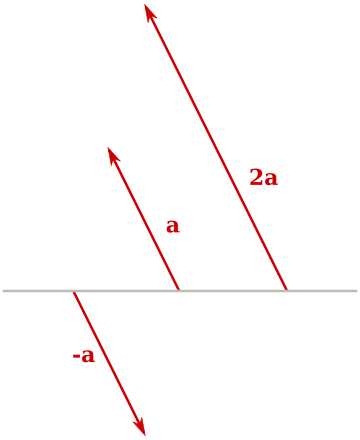
\includegraphics[width=0.98\textwidth]{./images/schematics/vector_multiplication_with_scalar_1.png}\\
   \end{center}
  \end{column}
  \begin{column}{0.55\textwidth}
     Let $\vec{A} = \Big( A_x, A_y, A_z \Big)$.\\
     \vspace{0.3cm}
     Then
     \begin{equation*}
       \lambda \vec{A} = \lambda \Big( A_x, A_y, A_z \Big) =
         \Big(\lambda A_x, \lambda A_y, \lambda A_z \Big)
     \end{equation*}
  \end{column}
\end{columns}

\end{frame}

%
%
%

\begin{frame}{Reminder: Dot product $\vec{A} \cdot \vec{B}$ of two vectors $\vec{A}$, $\vec{B}$}

Dot product $\vec{A} \cdot \vec{B}$ of two vectors $\vec{A}$, $\vec{B}$ is defined as
\begin{equation*}
  \vec{A} \cdot \vec{B} = A_{x} B_{x} + A_{y} B_{y} + A_{z} B_{z}
\end{equation*}
i.e. as the sum of the products of the x, y and z components of $\vec{A}$ and $\vec{B}$.\\
\vspace{0.3cm}

It can also be written as
\begin{equation*}
  \vec{A} \cdot \vec{B} =  |\vec{A}| |\vec{B}| cos\theta
\end{equation*}
where $|\vec{A}| = \sqrt{A_x^2+A_y^2+A_z^2}$ (similarly for $|\vec{B}|$) and $\theta$ is the
angle between $\vec{A}$ and $\vec{B}$.
So, the dot product $\vec{A} \cdot \vec{B}$ is
product of the magnitude of $\vec{A}$ with the magnitude of the
projection of $\vec{B}$ along $\vec{A}$ (or vice versa).\\
\vspace{0.3cm}

Please note that the {\bf dot product $\vec{A} \cdot \vec{B}$ is scalar}.

\end{frame}

%
%
%

\begin{frame}{Reminder: Dot product $\vec{A} \cdot \vec{B}$ of two vectors $\vec{A}$, $\vec{B}$}

As we have seen, the dot product of two vectors $\vec{A}$, $\vec{B}$ can be written as
\begin{equation*}
  \vec{A} \cdot \vec{B} =  |\vec{A}| |\vec{B}| cos\theta
\end{equation*}

One can easily see that:
\begin{itemize}
 \item If $\vec{A}$ and $\vec{B}$ are perpendicular ($\theta=\pi/2$) then $\vec{A} \cdot \vec{B} = 0$.
 \item If $\vec{A}$ and $\vec{B}$ are collinear ($\theta=0$) then $\vec{A} \cdot \vec{B} =  |\vec{A}| |\vec{B}|$.
 \item The dot product of a vector $\vec{A}$ with itself is $\vec{A} \cdot \vec{A} =  |\vec{A}|^2$.
\end{itemize}

\vspace{0.3cm}

Note that the dot product is
\begin{itemize}
   \item distributive [ $\vec{A} \cdot \Big( \vec{B} + \vec{C} \Big) = \vec{A} \cdot \vec{B} + \vec{A} \cdot \vec{C}$ ], and
   \item commutative [ $\vec{A} \cdot \vec{B} = \vec{B} \cdot \vec{A}$ ].
\end{itemize}

\end{frame}


%
%
%

\begin{frame}{Reminder: Cross product $\vec{A} \times \vec{B}$ of two vectors $\vec{A}$, $\vec{B}$}

The cross product $\vec{A} \times \vec{B}$ of two vectors $\vec{A}$, $\vec{B}$ is defined as
\begin{equation*}
     \vec{A} \times \vec{B} =
       \left|
          \begin{array}{ccc}
             \hat{i} & \hat{j} & \hat{k} \\
             A_x     & A_y     & A_z     \\
             B_x     & B_y     & B_z     \\
          \end{array}
       \right| =
       (A_y B_z - A_z B_y) \hat{i} - (A_x B_z - A_z B_x) \hat{j} + (A_x B_y - A_y B_x) \hat{k}
\end{equation*}

\begin{columns}
  \begin{column}{0.30\textwidth}
   \begin{center}
     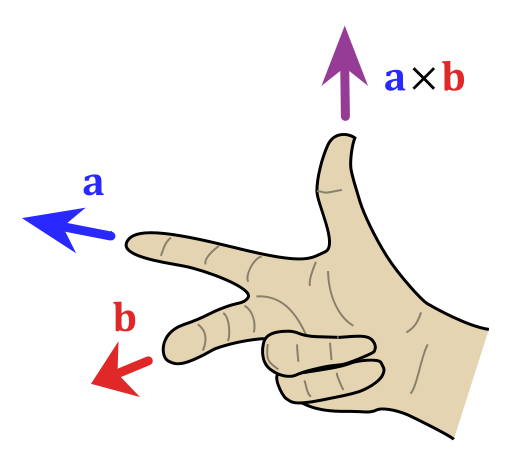
\includegraphics[width=0.98\textwidth]{./images/schematics/right_hand_rule_abc_3.png}\\
   \end{center}
  \end{column}
  \begin{column}{0.70\textwidth}
    It can also be written as
    \begin{equation*}
    \vec{A} \times \vec{B} = |\vec{A}| |\vec{B}| \; sin\theta \; \hat{n}
    \end{equation*}
    where $|\vec{A}| = \sqrt{A_x^2+A_y^2+A_z^2}$ (similarly for $|\vec{B}|$), $\theta$ is the
    angle between $\vec{A}$ and $\vec{B}$ and $\hat{n}$ is a unit vector perpendicular to both
    $\vec{A}$ and $\vec{B}$ as shown on the left.
  \end{column}
\end{columns}

\vspace{0.3cm}

Note that the {\bf cross product $\vec{A} \times \vec{B}$ is a vector} (actually, {\em pseudo}-vector).

\end{frame}


%
%
%

\begin{frame}{Reminder: Cross product $\vec{A} \times \vec{B}$ of two vectors $\vec{A}$, $\vec{B}$}

As we have seen, the cross product of two vectors $\vec{A}$, $\vec{B}$ can be written as
\begin{equation*}
   \vec{A} \times \vec{B} = |\vec{A}| |\vec{B}| \; sin\theta \; \hat{n}
\end{equation*}

One can easily see that:
\begin{itemize}
 \item If $\vec{A}$ and $\vec{B}$ are perpendicular ($\theta=\pi/2$) then $\vec{A} \times \vec{B} = |\vec{A}| |\vec{B}|$.
 \item If $\vec{A}$ and $\vec{B}$ are collinear ($\theta=0$) then $\vec{A} \times \vec{B} =  0$.
 \item The cross product of a vector $\vec{A}$ with itself is $\vec{A} \times \vec{A} = 0$.
\end{itemize}

\vspace{0.3cm}

Note that the cross product is
\begin{itemize}
   \item distributive [ $\vec{A} \times \Big( \vec{B} + \vec{C} \Big) = \vec{A} \times \vec{B} + \vec{A} \times \vec{C}$ ],
   \item not commutative [ $\vec{A} \times \vec{B} = - \Big( \vec{B} \times \vec{A} \Big)$ ].
\end{itemize}

\end{frame}


%
%
%

\begin{frame}{Reminder: Useful identities / Triple products}

{\bf Scalar triple product} $\vec{A} \cdot \Big( \vec{B} \times \vec{C} \Big)$:
\begin{equation*}
   \vec{A} \cdot \Big( \vec{B} \times \vec{C} \Big) =
     \vec{B} \cdot \Big( \vec{C} \times \vec{A} \Big) =
       \vec{C} \cdot \Big( \vec{A} \times \vec{B} \Big)
\end{equation*}
Notice how the order is preserved (cyclically) and that result is scalar.\\

\vspace{0.5cm}

{\bf Vector triple product} $\vec{A} \times \Big( \vec{B} \times \vec{C} \Big)$:
\begin{equation*}
   \vec{A} \times \Big( \vec{B} \times \vec{C} \Big) =
      \vec{B} \cdot \Big( \vec{A} \cdot \vec{C} \Big) -
      \vec{C} \cdot \Big( \vec{A} \cdot \vec{B} \Big)
\end{equation*}
This the so-called {\bf BAC-CAB rule}. Notice that result is a vector.\\

\vspace{0.5cm}

Higher vector products can be reduced by repeated applications of above.

\end{frame}

} % ending reminder

%
% Quiz
%

{
\problemslide

\begin{frame}{Quiz}

Recall that:
\begin{itemize}
  \item The product {\color{magenta} $\lambda \vec{A}$} of a vector $\vec{A}$ with a scalar $\lambda$
        {\color{magenta} is a vector}
  \item The {\bf dot product} {\color{magenta} $\vec{A} \cdot \vec{B}$} of two vectors $\vec{A}$, $\vec{B}$
        {\color{magenta} is a scalar}
  \item The {\bf cross product} {\color{magenta} $\vec{A} \times \vec{B}$} of two vectors $\vec{A}$, $\vec{B}$
        {\color{magenta} is a vector}
\end{itemize}

\vspace{0.4cm}

You should be able to answer the following:
\begin{blockexmplque}{Question}
 What is the product $(\vec{A} \cdot \vec{B}) \times \vec{C}$
 of three vectors $\vec{A}$, $\vec{B}$ and $\vec{C}$?\\
 Is it a scalar or a vector?
\end{blockexmplque}

\begin{blockexmplans}{Answer}
\noindent
\scalebox{1}[-1]{
%\reflectbox{
 \rotatebox[origin=c]{180}{
   \noindent
   \begin{minipage}[t]{\linewidth}
     The product is ill-formed and it means nothing. It is the cross product of a scalar with a vector!
   \end{minipage}%
 }
}
\end{blockexmplans}

\end{frame}

} % ending quiz


%
%
%

\begin{frame}{Coulomb's law}

Coulomb's law describes the {\bf electrical force between two charges}.\\

\vspace{0.4cm}

\begin{columns}
  \begin{column}{0.45\textwidth}
   \begin{center}
     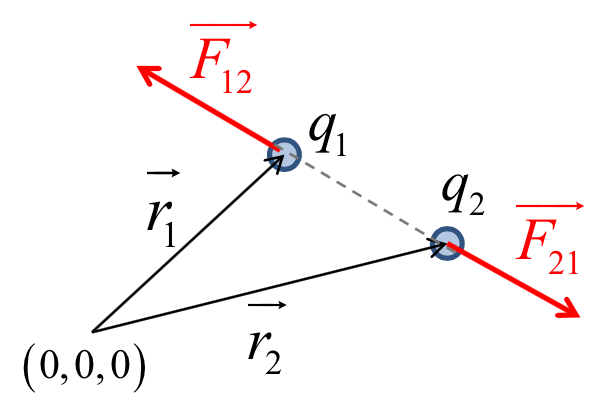
\includegraphics[width=0.98\textwidth]{./images/schematics/coulomb_force_2_like_charges.png}\\
     \vspace{0.3cm}
     {\it \small (drawn for like charges)}
   \end{center}
  \end{column}
  \begin{column}{0.55\textwidth}
     The force $\vec{F}_{12}$ exerted on test charge 1 by charge 2 (notice convention) is:\\
     {\Large
     \begin{equation*}
       \vec{F}_{12} = \frac{1}{4\pi\epsilon_0} \frac{q_1 q_2}{|\vec{r}_{1}-\vec{r}_{2}|^{2}} \hat{r}_{12}
     \end{equation*}
     }
     where:
        \begin{itemize}
          \item $\epsilon_0$ is the permittivity of free space ($\epsilon_0$ = 8.854 $\times 10^{-12}$ $C^2/Nm^2$), and
          \item $\hat{r}_{12}$ is a unit vector ($|\hat{r}_{12}|$=1) in the direction of $\vec{r}_{1}-\vec{r}_{2}$ (i.e. pointing from $q_2$ to $q_1$).
        \end{itemize}
  \end{column}
\end{columns}

\end{frame}


%
%
%

\begin{frame}{Coulomb's law}

\begin{columns}
  \begin{column}{0.60\textwidth}
     {\Large
     \begin{equation*}
       \vec{F}_{12} = \frac{1}{4\pi\epsilon_0} \frac{q_1 q_2}{|\vec{r}_{1}-\vec{r}_{2}|^{2}} \hat{r}_{12}
     \end{equation*}
     }
  \end{column}
  \begin{column}{0.40\textwidth}
   \begin{center}
     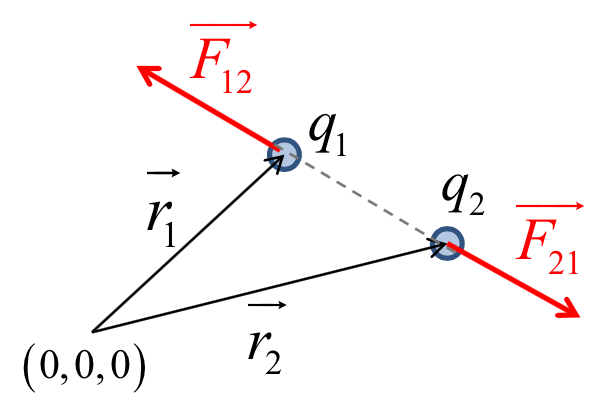
\includegraphics[width=0.90\textwidth]{./images/schematics/coulomb_force_2_like_charges.png}\\
     \vspace{0.3cm}
     {\it \small (drawn for like charges)}
   \end{center}
  \end{column}
\end{columns}

\underline{Observations:} The force
\begin{itemize}
  \item is proportional to the magnitude of each charge
  \item is inversely proportional to the square of the distance between charges
  \item has infinite range
  \item has a direction along the line connecting the two charges
  \item can be attractive or repulsive, depending on the charge signs
\end{itemize}

\end{frame}

%
%
%

\begin{frame}{Coulomb's law: Please notice the direction of $\vec{r}_1$ - $\vec{r}_2$}

  \begin{columns}
    \begin{column}{0.35\textwidth}
      \begin{center}
       {\color{red} \bf
        $\vec{r}_1$ - $\vec{r}_2$ is the vector pointing from $q_2$ to $q_1$},
       not the other way around (A common mistake!)\\
      \end{center}
      \begin{center}
        $\hat{r}_{12}$ is a unit vector along $\vec{r}_1$ - $\vec{r}_2$:
        \begin{equation*}
         \hat{r}_{12} = \widehat{r_1-r_2}
        \end{equation*}
      \end{center}
    \end{column}
    \begin{column}{0.65\textwidth}
      \begin{center}
        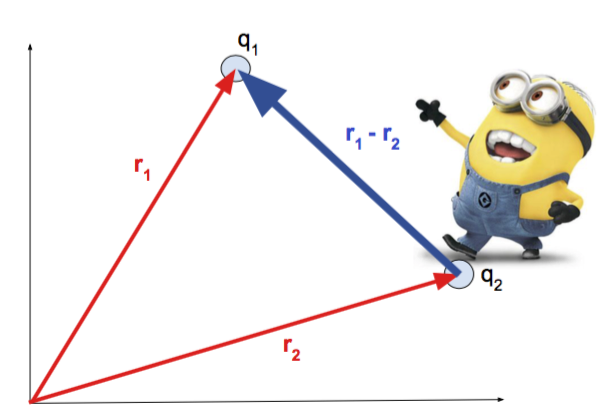
\includegraphics[width=0.95\textwidth]{./images/schematics/r1_r2_direction.png}\\
      \end{center}
    \end{column}
  \end{columns}

  \vspace{0.2cm}

  \begin{columns}
    \begin{column}{0.30\textwidth}
      \begin{equation*}
        \vec{F}_{12} = \frac{1}{4\pi\epsilon_0} \frac{q_1 q_2}{|\vec{r}_{1}-\vec{r}_{2}|^{2}} \hat{r}_{12}
      \end{equation*}
    \end{column}
    \begin{column}{0.70\textwidth}
        \begin{itemize}
          \item $\vec{F}_{12}$ points along $\hat{r}_{12}$ if $q_1 \cdot q_2 > 0$
          \item $\vec{F}_{12}$ has opposite direction from $\hat{r}_{12}$ if $q_1 \cdot q_2 < 0$
        \end{itemize}
    \end{column}
  \end{columns}

\end{frame}

%
%
%

\begin{frame}{Coulomb's law: Notice the difference between $\vec{F}_{12}$ and $\vec{F}_{21}$}

\begin{columns}
  \begin{column}{0.63\textwidth}
     {
     \begin{equation*}
       \vec{F}_{12} = \frac{1}{4\pi\epsilon_0} \frac{q_1 q_2}{|\vec{r}_{1}-\vec{r}_{2}|^{2}} \hat{r}_{12}
     \end{equation*}
     \begin{equation*}
       \vec{F}_{21} = \frac{1}{4\pi\epsilon_0} \frac{q_2 q_1}{|\vec{r}_{2}-\vec{r}_{1}|^{2}} \hat{r}_{21}
                    = \frac{1}{4\pi\epsilon_0} \frac{q_1 q_2}{|\vec{r}_{1}-\vec{r}_{2}|^{2}} (-\hat{r}_{12})
     \end{equation*}
     }
  \end{column}
  \begin{column}{0.37\textwidth}
   \begin{center}
     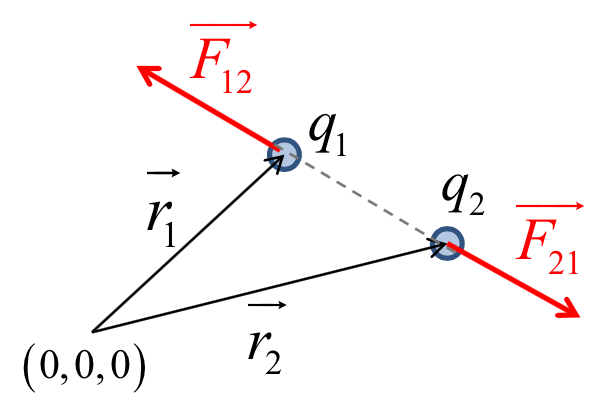
\includegraphics[width=0.90\textwidth]{./images/schematics/coulomb_force_2_like_charges.png}\\
     \vspace{0.3cm}
     {\it \small (drawn for like charges)}
   \end{center}
  \end{column}
\end{columns}

\begin{equation*}
 \vec{F}_{21} = - \vec{F}_{12} \;\;\;
 \begin{cases}
    \; \vec{F}_{12} \text{ is the force exerted on test charge 1 by charge 2}\\
    \\
    \; \vec{F}_{21} \text{ is the force exerted on test charge 2 by charge 1}
 \end{cases}
\end{equation*}

\begin{center}
{\small
Take notice of the convention and the relative minus sign between $\vec{F}_{12}$ and $\vec{F}_{21}$.\\
A common mistake is to calculate  $\vec{F}_{12}$ when $\vec{F}_{21}$ is asked (or vice versa).
}
\end{center}

\end{frame}


%
%
%

\begin{frame}{Coulomb's law: $\hat{r}/|\vec{r}\;|^2$ vs $\vec{r}/|\vec{r}\;|^3$}

We wrote the force exerted on test charge 1 by a test charge 2 ($\vec{F}_{12}$) as:\\
{\Large
\begin{equation*}
   \vec{F}_{12} =
      \frac{1}{4\pi\epsilon_0}
      \frac{q_1 q_2}{|\vec{r}_{1}-\vec{r}_{2}|^{\color{red}2}}
      {\color{red} \hat{(r_{1}-r_{2})}}
\end{equation*}
}
\vspace{0.2cm}

Sometimes, we will also be writing it as:\\
{\Large
\begin{equation*}
   \vec{F}_{12} =
      \frac{1}{4\pi\epsilon_0}
      \frac{q_1 q_2}{|\vec{r}_{1}-\vec{r}_{2}|^{\color{red}3}}
      {\color{red} (\vec{r}_{1}-\vec{r}_{2})}
\end{equation*}
}
\vspace{0.2cm}

The two expressions are {\bf completely equivalent}.\\
\vspace{0.2cm}

{\small
A surprising large number of students doesn't see that, and several students mix the two equations
(e.g. using a unit vector $\hat{r}_{12}$ but then a cube power of $|\vec{r}_{1}-\vec{r}_{2}|$).
If you too are confused, please study the next slide carefully.
}

\end{frame}

%
%
%

\begin{frame}{Coulomb's law: $\hat{r}/|\vec{r}\;|^2$ vs $\vec{r}/|\vec{r}\;|^3$}

\begin{center}
$\displaystyle \vec{F}_{12} = \frac{1}{4\pi\epsilon_0} \frac{q_1 q_2}{|\vec{r}_{1}-\vec{r}_{2}|^{2}} \hat{r}_{12}$
$\;\;\;$
is the same as
$\;\;\;$
$\displaystyle \vec{F}_{12} = \frac{1}{4\pi\epsilon_0} \frac{q_1 q_2}{|\vec{r}_{1}-\vec{r}_{2}|^{3}} \vec{r}_{12}$\\
\end{center}

\vspace{0.4cm}

Notice that:
\begin{equation*}
   \frac{\vec{r}}{r^3} =
   \frac{r\cdot\hat{r}}{r^3} =
   \frac{\hat{r}}{r^2}
\end{equation*}

where:
\begin{itemize}
  \item $\vec{r}$ is a vector (a quantity that is characterised both by a magnitude and a direction),
  \item r is the magnitude of $\vec{r}$, and
  \item $\hat{r}$ is a unit vector along $\vec{r}$ (has the same direction as $\vec{r}$, but its magnitude is 1).
\end{itemize}

\vspace{0.3cm}

If you still don't see the above equivalence, please come and talk to me.

\end{frame}

%
%
%

\begin{frame}{Coulomb's law}

\begin{columns}[t]
  \begin{column}{0.20\textwidth}
   \begin{center}
     \vspace{0.2cm}
     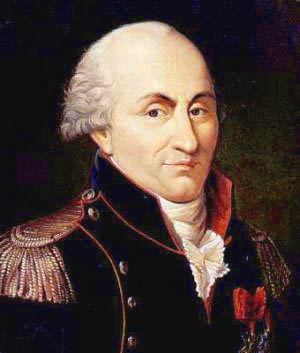
\includegraphics[width=0.90\textwidth]{./images/people/coulomb.jpg}\\
     {\scriptsize
      Charles-Augustin de Coulomb (1736-1806), French physicist.\\
      \vspace{0.2cm}
      His law was included in his 1785 publication
      Premier M\'emoire sur l'\'Electricit\'e et le Magn\'etisme.\\
     }
   \end{center}
  \end{column}
  \begin{column}{0.55\textwidth}
    \begin{center}
      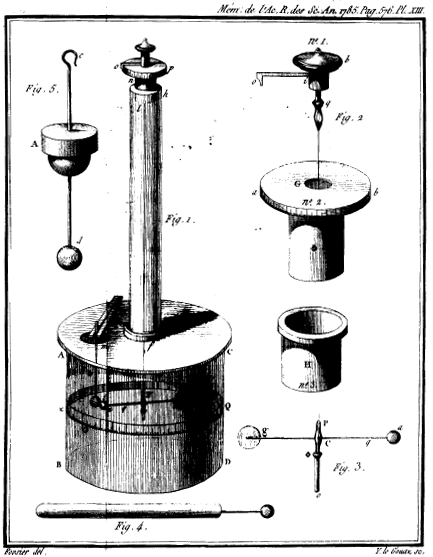
\includegraphics[width=0.80\textwidth]{./images/schematics/coulomb_torsion_balance.png}\\
    \end{center}
  \end{column}
  \begin{column}{0.25\textwidth}
   \begin{center}
    \vspace{0.2cm}
    {\scriptsize
     Coulomb deduced his law using a {\bf torsion balance} experiment:\\
     \vspace{0.2cm}
     An insulating rod, with a metal-coated (charged) ball attached on one end,
     is suspended by a silk fiber which acts as a weak torsion spring.
     A second charged ball brought near to the first one twists the silk fiber by a certain angle.
     The electrical force can be deduced from the force it took to twist the fiber as much as it did.\\
    }
   \end{center}
  \end{column}
\end{columns}

\end{frame}

%
%
%

\begin{frame}{Coulomb's law}

\begin{columns}[t]
  \begin{column}{0.20\textwidth}
   \begin{center}
     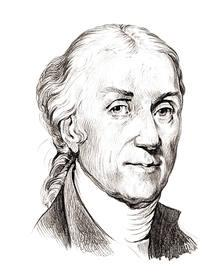
\includegraphics[width=0.90\textwidth]{./images/people/cavendish.jpg}\\
     {\scriptsize
      Henry Cavendish (1731-1810), British physicist.\\
     }
   \end{center}
  \end{column}
  \begin{column}{0.80\textwidth}
    \begin{itemize}
    {\small
     \item
     In the early 1770's, {\bf Henry Cavendish}, an English physicist,
     had already discovered the dependence of the electrical force
     upon the distance and charge. He never published it!
     \begin{itemize}
     {\scriptsize
      \item Cavendish measured that the force was inversely
            proportional to {\color{red} n = 2.00 $\pm$ 0.02}
      \item His experiment (using 2 concentric conducting rings) was a
            direct application of Gauss' law (published a century later)!
     }
     \end{itemize}
     \vspace{0.2cm}
     \item
     And others before Cavendish (Daniel Bernoulli, Alessandro Volta,
     Joseph Priestley, John Robinson) either suspected the
     inverse square law or performed measurements.\\
     \vspace{0.2cm}
     \item
     Later, {\bf Maxwell}, refining the Cavendish technique measured
     {\color{red} n = 2.0 $\pm$ 0.00005} [Maxwell, Vol 1,  p. 80]\\
     \vspace{0.2cm}
     \item
     In 1936 {\bf Plimpton and Lawton} found that Coulomb's exponent
     {\color{red} differs from two by less than one part in a billion!}
    }
    \end{itemize}
  \end{column}
\end{columns}

\end{frame}


%
% Quiz
%

{
\problemslide

%
%
%

\begin{frame}{Coulomb's law / Quiz}

The electrical force like the gravitational force, but `a {\bf billion - billion - billion - billion} times stronger' [Feynman Lectures].

\begin{blockexmplque}{\small Question [Feynman Lectures]}
{\scriptsize
  Within our body we have both positive charges (protons) and negative charges (electrons) in equal amounts.
  The attractive and repulsive forces "cancel out" so we do not attract or repel each other electrically.
  If our bodies had just 1\% more protons than electrons,
  the repelling force at a distance of an arm's length would be enough to lift a weight equal to that of
  \begin{itemize}
  {\scriptsize
    \item yourself?
    \item everybody in this class?
    \item everything in this city?
    \item the moon?
    \item more??
  }
  \end{itemize}
}
\end{blockexmplque}

\begin{blockexmplans}{\small Answer}
\noindent
\scalebox{1}[-1]{
%\reflectbox{
 \rotatebox[origin=c]{180}{
   \noindent
   \begin{minipage}[t]{\linewidth}
   {\scriptsize
     Actually, the repelling force at a distance of an arm's length would be enough to lift a weight equal to that of the entire Earth!
   }
   \end{minipage}%
 }
}
\end{blockexmplans}

\end{frame}

}

%
%
%

\begin{frame}{Note on e/m units}

\begin{itemize}
\item
  There is arbitrariness in the choice of the fundamental units.
  \begin{itemize}
   \item
     Traditionally, we take the mass, length and time as basic units (but this is not necessary and other choices are also in use).
  \end{itemize}
\vspace{0.2cm}
\item
   Take Coulomb's law:
   \begin{equation*}
        |\vec{F}_{12}| \propto \frac{q_1 q_2}{|\vec{r}_{1}-\vec{r}_{2}|^{2}}
    \end{equation*}
    \begin{itemize}
      \item
        the constant of proportionality is automatically defined if the magnitude and dimensions of the unit of charge has been defined in advance, or
       \item
        one can choose the constant of proportionality arbitrarily and then use Coulomb's law to define the unit of charge.
    \end{itemize}
\vspace{0.2cm}
\item
  For e/m quantities there is no compelling tradition.
  \begin{itemize}
   \item
    Many systems of units:
    {\bf electrostatic} (esu), {\bf electromagnetic} (emu),
    {\bf Gaussian}, {\bf Heaviside - Lorentz}, {\bf SI / rationalised}, ...
   \end{itemize}
\end{itemize}

\end{frame}

%
%
%

\begin{frame}{Note on e/m units}

\begin{itemize}
\item
 What's more, various e/m equations look somewhat different in different systems.

 {\scriptsize
   \begin{equation*}
     |\vec{F}_{12}| = \frac{q_1 q_2}{|\vec{r}_{1}-\vec{r}_{2}|^{2}} \;\; {\color{magenta}(Gaussian)},  \;\;
     |\vec{F}_{12}| = \frac{1}{4 \pi \epsilon_0} \frac{q_1 q_2}{|\vec{r}_{1}-\vec{r}_{2}|^{2}} \;\; {\color{magenta}(SI)},  \;\;
     |\vec{F}_{12}| = \frac{1}{4 \pi} \frac{q_1 q_2}{|\vec{r}_{1}-\vec{r}_{2}|^{2}} \;\; {\color{magenta}(HL)}
   \end{equation*}
 }

\item
  Different popular textbooks use different systems of units: A source of confusion!

\item
  If you are interested in the issue of systems of units for e/m quantities, glance though the Appendix of J.D.Jackson's Classical Electrodynamics (ISBN-13: 978-0471309321).

\item
 The Gaussian and SI/rationalised are the most commonly used system of units.

\item
 The slides, as well as in all recommended textbooks, the SI/rationalised system of units is used.

\end{itemize}

\end{frame}

%
% Worked example
%

{
\problemslide

%
%
%

\begin{frame}{Worked example}

\begin{blockexmplque}{Question}
Find the force on charge $q_1$, 20 ${\mu}C$, due to charge $q_2$, -300 ${\mu}C$,
where $q_1$ is at position $\vec{r}_{1}$ = (0, 1, 2) m and $q_2$ is at position $\vec{r}_{2}$ = (2, 0, 0).
\end{blockexmplque}
\vspace{0.4cm}

As we have seen, the force on charge $q_1$  due to charge $q_2$ is:
\begin{equation*}
  \displaystyle
   \vec{F}_{12} = \frac{1}{4\pi\epsilon_0} \frac{q_1 q_2}{|\vec{r}_{1}-\vec{r}_{2}|^{3}} (\vec{r}_{1}-\vec{r}_{2})
\end{equation*}

The position $\vec{r}_{1}-\vec{r}_{2}$  of $q_1$ relative to $q_2$ is:
\begin{equation*}
  \displaystyle
   \vec{r}_{1}-\vec{r}_{2} =  (0, 1, 2) \; m - (2, 0, 0) \; m = (-2, 1, 2) \; m
\end{equation*}

The magnitude of $\vec{r}_{1}-\vec{r}_{2}$ is:
\begin{equation*}
  \displaystyle
   |\vec{r}_{1}-\vec{r}_{2}| =  \sqrt{ (-2)^2 + 1^2 + 2^2} \; m = \sqrt{9} \; m = 3 \; m
\end{equation*}

\end{frame}

%
%
%

\begin{frame}{Worked example}

Therefore:
\begin{equation*}
  \displaystyle
   \vec{F}_{12} = \frac{1}{4\pi\epsilon_0} \frac{q_1 q_2}{|\vec{r}_{1}-\vec{r}_{2}|^{3}} (\vec{r}_{1}-\vec{r}_{2}) \Rightarrow
\end{equation*}
\begin{equation*}
  \displaystyle
    \vec{F}_{12} =
              ( 9.0 \times 10^9 \; \frac{N \cdot m^2}{C^2}) \cdot
              \frac{(20 \times 10^{-6} \; C) (-300 \times 10^{-6} \; C)}{(3\;m)^3} \cdot (-2, 1, 2) \; m \Rightarrow
\end{equation*}
\begin{equation*}
  \displaystyle
    \vec{F}_{12} =
              ( 9.0 \times 10^9 \; \frac{N \cdot m^2}{C^2}) \cdot
              \frac{-6000 \times 10^{-12} \; C^2}{27\;m^3} \cdot (-2, 1, 2) \; m \Rightarrow
\end{equation*}
\begin{equation*}
  \displaystyle
    \vec{F}_{12} =
        - \frac{(9.0 \times 10^9) \cdot (6 \times 10^{-9})}{27} \cdot (-2, 1, 2) \; N \Rightarrow
\end{equation*}
\begin{equation*}
  \displaystyle
    \vec{F}_{12} =
        - \frac{54}{27} \cdot (-2, 1, 2) \; N =  -2 \cdot (-2, 1, 2) \; N \Rightarrow
\end{equation*}
\begin{equation*}
  \displaystyle
    \vec{F}_{12} = (4, -2, -4) \; N
\end{equation*}

\end{frame}


} % Example


%
%
%

\begin{frame}{Superposition principle}

The forces exerted by several charges on a test charge superimpose each other undisturbed:
The total force is the vector sum of forces.\\
\vspace{0.2cm}
\begin{columns}
  \begin{column}{0.35\textwidth}
   \begin{center}
     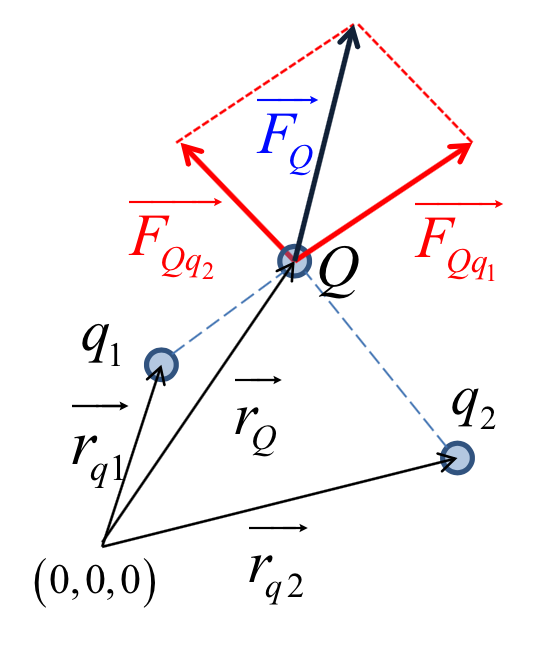
\includegraphics[width=0.95\textwidth]{./images/schematics/coulomb_force_superposition.png}\\
     {\it \small (drawn for like charges)}
   \end{center}
  \end{column}
  \begin{column}{0.65\textwidth}
     The total force $\vec{F}_{Q}$ exerted on test charge Q by test charges $q_1$, $q_2$ is:
     \begin{equation*}
       \vec{F}_{Q} = \sum_{i=1}^{2} F_{Qq_{i}} \Rightarrow
     \end{equation*}
     \begin{equation*}
       \vec{F}_{Q} = \sum_{i=1}^{2} \frac{1}{4\pi\epsilon_0}
         \frac{Q q_i}{|\vec{r}_{Q}-\vec{r}_{q_{i}}|^{2}} \hat{r}_{Qq_{i}} \Rightarrow
     \end{equation*}
     \begin{equation*}
        \vec{F}_{Q} = \sum_{i=1}^{2} \frac{1}{4\pi\epsilon_0}
          \frac{Q q_i}{|\vec{r}_{Q}-\vec{r}_{q_{i}}|^{3}} (\vec{r}_{Q}-\vec{r}_{q_{i}})
     \end{equation*}
  \end{column}
\end{columns}

\end{frame}

%
%
%

\begin{frame}[t]{Superposition principle}

{\bf Superposition is not a logical necessity, but an experimental fact}.\\
\vspace{0.3cm}
Here is how things could have been different:\\
\vspace{0.2cm}

\begin{itemize}
\item
  Example 1:
  {\color{magenta} If the electromagnetic force were proportional to the square of the total source charge} [Griffiths].\\
  \vspace{0.2cm}
  Then, obviously
  \begin{equation*}
    Q^2 (q_1 + q_2)^2 \ne Q^2 q_1^2 +  Q^2 q_2^2
  \end{equation*}
\end{itemize}

\end{frame}

%
%
%

\begin{frame}[t]{Superposition principle}

{\bf Superposition is not a logical necessity, but an experimental fact}.\\
\vspace{0.3cm}
Here is how things could have been different:\\
\vspace{0.2cm}

\begin{itemize}
\item
Example 2:
  {\color{magenta} If there were many-body forces} [Greiner].\\
  \vspace{0.2cm}
  {\small
  The Coulomb force between charges is merely a {\bf 2-body force}:
  This means that the force between two charges is undisturbed from the presence
  of other bodies and many-body forces do not occur. \\
  \vspace{0.2cm}
  A many-body force is one where the force between bodies 1 and 2 would also
  depend on the positions and charges of other bodies.
  Below is an example of a hypothetical 3-body force
  ($r_s$ is the centre of gravity between $q_1$, $q_2$):\\
  }
  {\Large
  \begin{equation*}
    \vec{F}_{12} = \frac{q_1 q_2}{4\pi\epsilon_0}
       \frac{\vec{r_1} - \vec{r_2}}
            {|(\vec{r_1} - \vec{r_2}) \Big( 1 + \frac{q_3^2}{q_1 q_2} \cdot \frac{|\vec{r_1} - \vec{r_2}|}{|\vec{r_s} - \vec{r_3}|} \Big)|^3}
  \end{equation*}
  }
\end{itemize}

\end{frame}

%
%
%

\begin{frame}{Coulomb force due to an array of charges $q_1$, $q_2$, ..., $q_n$}

So, starting from the basic Coulomb force between two charges and using the superposition principle,
we can compute the total force exerted on a charge Q, by an array of charges $q_1$, $q_2$, ..., $q_n$.\\

\vspace{0.2cm}

The total force on Q is the vector sum of all forces due to each of $q_1$, $q_2$, ..., $q_n$ individually:

\begin{equation*}
   \vec{F}_{Q} = \sum_{i=1}^{n} \frac{1}{4\pi\epsilon_0}
       \frac{Q q_i}{|\vec{r}_{Q}-\vec{r}_{q_{i}}|^{3}} (\vec{r}_{Q}-\vec{r}_{q_{i}})
\end{equation*}

\end{frame}

%
% Quiz
%

{
\problemslide

\begin{frame}{Quiz}

Recall Coulomb's force and the superposition principle.\\
\vspace{0.2cm}

\begin{blockexmplque}{Question}
  The figure shows two protons (symbol p) and one electron (symbol e) on an axis.
  \begin{center}
    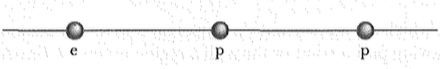
\includegraphics[width=0.75\textwidth]{./images/problems/lect1_quiz_epp_charges.png}
  \end{center}
  What is the direction of
  \begin{enumerate}
    {\small
    \item the electrostatic force on the central proton due to the electron,
    \item the electrostatic force on the central proton due to the other proton, and
    \item the net electrostatic force on the central proton?\\
    }
  \end{enumerate}

\end{blockexmplque}

% \begin{blockexmplans}{Answer}
% \noindent
% \scalebox{1}[-1]{
% %\reflectbox{
%  \rotatebox[origin=c]{180}{
%    \noindent
%    \begin{minipage}[t]{\linewidth}
%      The product is ill-formed and it means nothing. It is the cross product of a scalar with a vector!
%    \end{minipage}%
%  }
% }
% \end{blockexmplans}

\end{frame}

} % ending quiz


%
% Worked example
%

{
\problemslide

%
%
%

\begin{frame}{Worked example }

\begin{blockexmplque}{Question}
\begin{columns}
  \begin{column}{0.25\textwidth}
   \begin{center}
     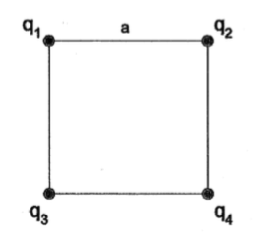
\includegraphics[width=0.98\textwidth]{./images/problems/lect1_array_of_4_charges.png}
   \end{center}
  \end{column}
  \begin{column}{0.75\textwidth}
     Four charges are located at the four corners of a square of side a.
     The charges are $\displaystyle q1 = q4 = Q$ and $\displaystyle q2 = q3 = q$.
     What is the ratio Q/q if the net electrostatic force on particle 1 is zero?
  \end{column}
\end{columns}
\end{blockexmplque}

\vspace{0.1cm}

The Coulomb force exerted on charge $q_i$ due to a charge $q_j$ at
distance $\vec{r}$ is given by:
\begin{equation*}
   \vec{F}_{ij} = \frac{1}{4\pi \epsilon_0} \cdot \frac{q_i q_j}{|\vec{r}|^3} \vec{r}
\end{equation*}

Take the x-axis to be parallel with the line connecting the charges
$q_1$ and $q_2$, and pointing from $q_1$ to $q_2$.
We will calculate the x-component of the force exerted on $q_1$
due to each of $q_2$, $q_3$ and $q_4$.

\end{frame}


%
%
%

\begin{frame}{Worked example }

\begin{equation*}
   F_{12;x} =
      \frac{1}{4\pi \epsilon_0} \cdot \frac{q_1 q_2}{a^2}  =
      \frac{1}{4\pi \epsilon_0} \cdot \frac{Qq}{a^2}
\end{equation*}

\begin{equation*}
   F_{13;x} = 0
\end{equation*}

\begin{equation*}
   F_{14;x} =
     \frac{1}{4\pi \epsilon_0} \cdot \frac{q_1 q_4}{(\sqrt{2} \; a)^2} \cdot cos\Big( \frac{\pi}{4} \Big) =
     \frac{1}{4\pi \epsilon_0} \cdot \frac{Q^2}{2a^2} \cdot \frac{1}{\sqrt{2}}
\end{equation*}

Thefore, the x-component of the total force experienced by $q_1$ is:
\begin{equation*}
   F_{1;x} = F_{12;x} + F_{13;x} + F_{14;x} =
    \frac{1}{4\pi \epsilon_0} \cdot
    \bigg\{
        \frac{Q^2}{2\sqrt{2}a^2}
        +\frac{qQ}{a^2}
    \bigg\}
\end{equation*}

Setting $F_{1;x} = 0$, we have:
\begin{equation*}
     \frac{Q^2}{2\sqrt{2}a^2} +\frac{qQ}{a^2} = 0 \Rightarrow
     \frac{Q}{2\sqrt{2}} +q = 0 \Rightarrow
     \frac{Q}{q} = -2\sqrt{2} \Rightarrow
     \frac{Q}{q} = -2.83
\end{equation*}

\end{frame}


} % Example



%
%
%

\begin{frame}{Continuous charge distributions}

To describe complex distributions of charges, we use the concept of {\bf charge density}.
It describes the amount of charge per unit volume, area or length.\\
\vspace{0.2cm}
\begin{itemize}
\item
If charge Q is distributed continuously over a volume, the (volume) charge density $\rho(\vec{r})$ is given by:
\begin{equation*}
   {\color{red} \rho(\vec{r}) = \frac{dQ(\vec{r})}{d\tau} } \Rightarrow
   Q = \int_{volume} d\tau \; \rho(\vec{r})
\end{equation*}
\item
If charge Q is distributed continuously over a surface, use surface charge density ($\sigma(\vec{r})$)
\begin{equation*}
   {\color{red} \sigma(\vec{r}) = \frac{dQ(\vec{r})}{dS} } \Rightarrow
   Q = \int_{area} dS \; \sigma(\vec{r})
\end{equation*}
\item
Charge distributed (continuously) along a line: use linear charge density ($\lambda(\vec{r})$)
\begin{equation*}
   {\color{red} \lambda(\vec{r}) = \frac{dQ(\vec{r})}{dl} } \Rightarrow
   Q = \int_{line} dl \; \lambda(\vec{r})
\end{equation*}
\end{itemize}

\end{frame}

%
%
%

\begin{frame}{Coulomb force due to a continuous charge distribution}

Here, we are considering charge distributed in a volume
(similarly for charge distributed on a surface or along a line).

\begin{columns}
  \begin{column}{0.60\textwidth}
    \begin{center}
      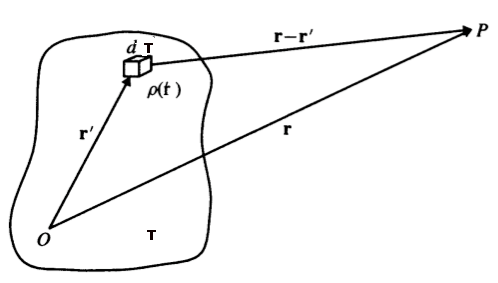
\includegraphics[width=0.95\textwidth]{./images/schematics/charge_distribution_3d_tau.png}\\
    \end{center}
  \end{column}
  \begin{column}{0.40\textwidth}
     We will start from the discrete case, and do the following substitutions:
     \begin{itemize}
       \item $\vec{r}_{q_i} \rightarrow$ $\pvec{r}'$
       \item $\vec{r}_{Q} \rightarrow$ $\vec{r}$
       \item $q_i \rightarrow d\tau^{\prime} \rho(\pvec{r}')$
       \item $\sum \rightarrow \int$
     \end{itemize}
  \end{column}
\end{columns}

\vspace{0.1cm}
We no longer enumerate positions with the charge ID, and replace the sum / discrete
charges with integral / charge density.
Therefore:
\begin{equation*}
   \vec{F}_{Q} = \frac{Q}{4\pi\epsilon_0} \sum_{i=1}^{n}
      \frac{q_i}{|\vec{r}_{Q}-\vec{r}_{q_{i}}|^{3}} (\vec{r}_{Q}-\vec{r}_{q_{i}})
   \xRightarrow{\sum\rightarrow\int}
   \vec{F}_{Q} = \frac{Q}{4\pi\epsilon_0} \int_{\tau}
      d\tau^{\prime} \frac{\rho({\pvec{r}'})}{|\vec{r}-\pvec{r}'|^{3}} (\vec{r}-\pvec{r}')
\end{equation*}

\end{frame}


%
%
%

\begin{frame}{Oddities of Coulomb's force}

Coulomb's force, as we introduced it, has some oddities:\\
\vspace{0.5cm}
\begin{itemize}
  \item {\bf Action at a distance}
    \begin{itemize}
       \item In early theories, all physical interaction was reduced to {\em collision}.
       \item But what is the medium that carries Coulomb's force?
    \end{itemize}
  \vspace{0.3cm}
  \item {\bf Instantaneous}
    \begin{itemize}
       \item But nothing, including the influence of one charge on another, can travel
             faster than the speed of light.
    \end{itemize}
\end{itemize}

\end{frame}


% starting reminder
{
\reminderslide

\begin{frame}{Reminder: Fields}

{\bf A {\em field} is a physical quantity that permeates all space!}\\
\vspace{0.1cm}
If that physical quantity
\begin{itemize}
  \item is just a number (a scalar) we have a {\bf scalar field}
  \item has magnitute and direction (is a vector) we have a {\bf vector field}
\end{itemize}
\begin{columns}[t]
  \begin{column}{0.47\textwidth}
   \begin{center}
     {\it \scriptsize Temperature map (a scalar field)}\\
     \vspace{0.3cm}
     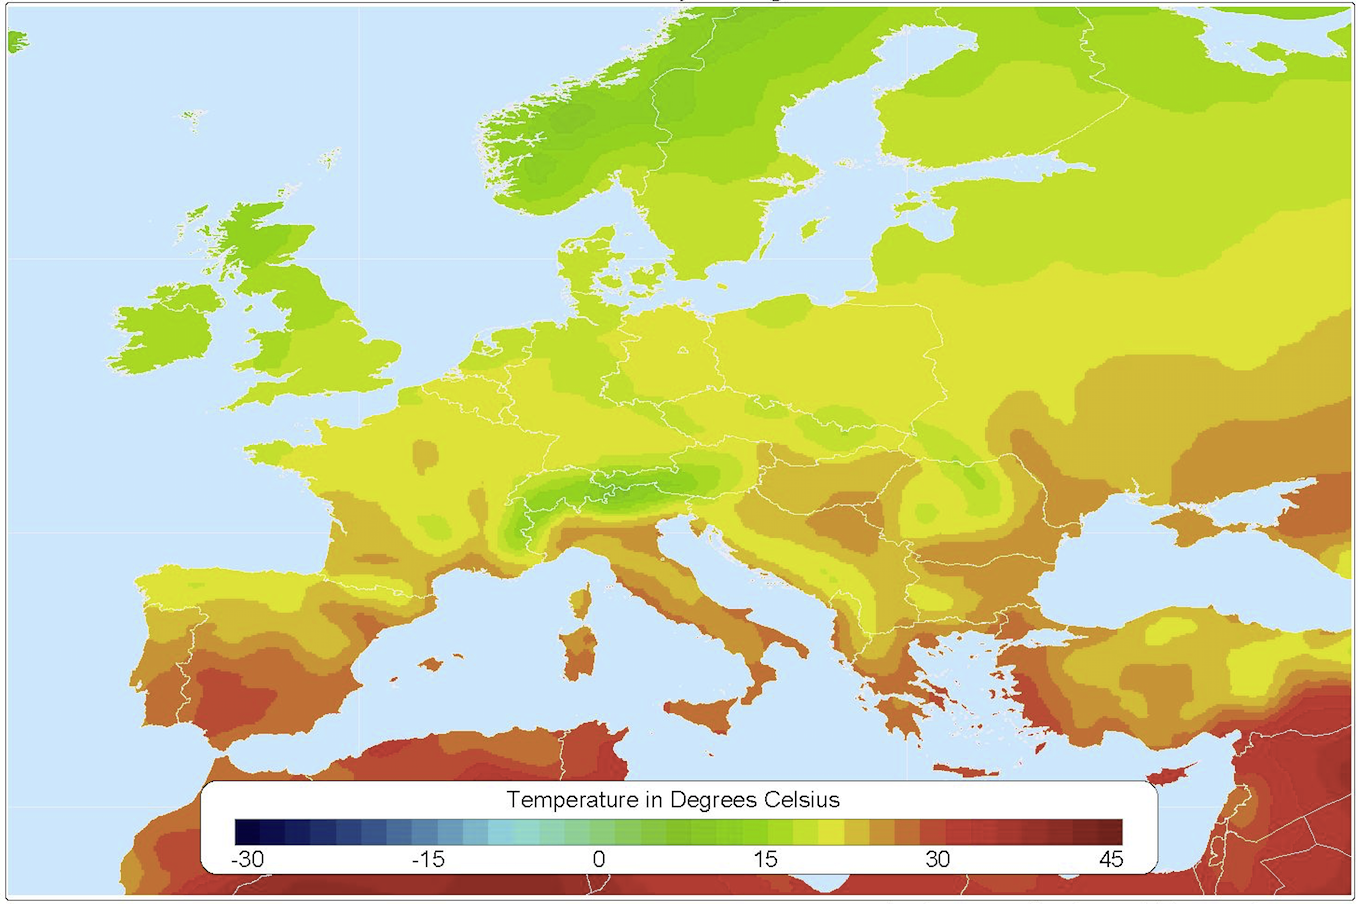
\includegraphics[width=0.80\textwidth]{./images/schematics/field_scalar_eu_temp_map.png}\\
   \end{center}
  \end{column}
  \begin{column}{0.53\textwidth}
   \begin{center}
     {\it \scriptsize Wind map (a vector field)}\\
     \vspace{0.3cm}
     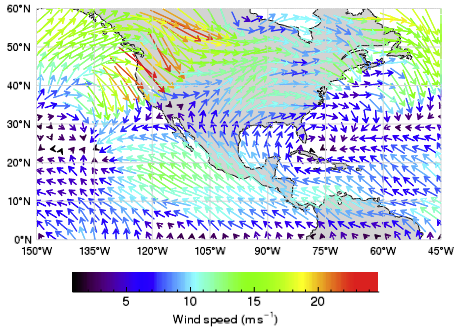
\includegraphics[width=0.75\textwidth]{./images/schematics/field_vector_us_wind_map.png}\\
   \end{center}
  \end{column}
\end{columns}

In electromagnetism, we will see several scalar and vector fields.

\end{frame}

} % ending reminder


%
%
%

\begin{frame}{Electric field}

\begin{center}
 It is useful to introduce a new concept: The {\bf electric field} $\vec{E}$
\end{center}
\begin{columns}
  \begin{column}{0.50\textwidth}
   \begin{center}
     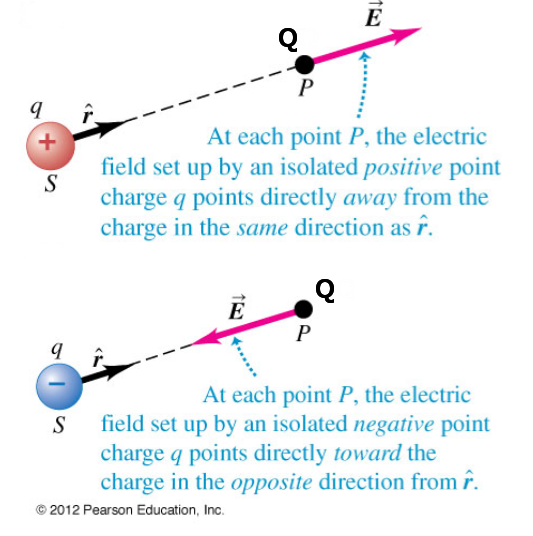
\includegraphics[width=0.98\textwidth]{./images/schematics/electric_field_2_charges_1.png}\\
   \end{center}
  \end{column}
  \begin{column}{0.50\textwidth}
  {\small
     Defined as force exerted on test charge Q, placed in position r, per unit charge.\\
     \begin{equation*}
       \vec{E}(\vec{r}) = \frac{\vec{F}_Q(\vec{r})}{Q}
     \end{equation*}
     $\vec{E}$ is a field - it {\bf permeates all space}.\\
     A charge creates an electric field around it. Other charges feel an electrical force because
     of the existence of this field.\\
     \vspace{0.1cm}
     Here we consider stationary charges (field sources):
     $\vec{E}$ doesn't depend on t.\\
     \vspace{0.2cm}
     $\vec{E}$ has units of $NC^{-1}$ (= $Vm^{-1}$).
  }
  \end{column}
\end{columns}
\end{frame}


%
%
%

\begin{frame}{Electric field}

The electric field was defined as the force exerted on a test charge, placed in position $\vec{r}$, per unit charge.
\begin{equation*}
  \vec{E}(\vec{r}) = \frac{\vec{F}_Q(\vec{r})}{Q}
\end{equation*}
\vspace{0.3cm}
\underline{Be careful with this definition!}\\
\begin{itemize}
  \item The electric field times the charge of a body  does not necessarily give us the force exerted on that body.
  \item If that charge is too large, it may disrupt the array of charges creating the electric field.
  \item The electric field (magnitude and direction) is the {\bf constant limiting value}
        of the force/charge ratio {\bf as the charge becomes smaller and smaller}.
\end{itemize}
\end{frame}


%
%
%

\begin{frame}{Electric field due to an array of charges}

\begin{columns}
  \begin{column}{0.60\textwidth}
   \begin{center}
     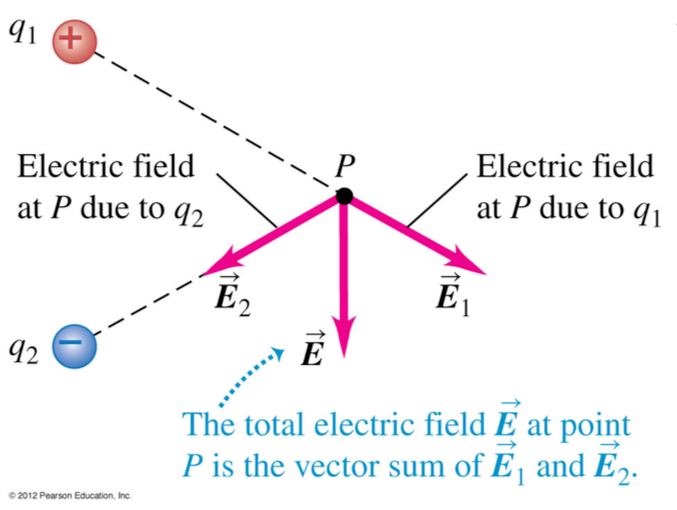
\includegraphics[width=0.95\textwidth]{./images/schematics/electric_field_superposition.png}\\
   \end{center}
  \end{column}
  \begin{column}{0.40\textwidth}
     What about the electric {\bf field created by an array of charges}?\\
     \vspace{0.4cm}
     The {\bf superposition principle} applies.
  \end{column}
\end{columns}
\vspace{0.2cm}
The electric field at position P (where test charge Q is inserted) is given by:
\begin{equation*}
\displaystyle
   \vec{E} = \frac{\vec{F}_Q}{Q} = \frac{\sum_{i=1}^{n} \vec{F}_Qq_{i}}{Q} = \sum_{i=1}^{n} \vec{E}_i
\end{equation*}

\end{frame}


%
%
%

\begin{frame}{Visualising the electric field}

It was easy to visualise the electric force (a vector).
But how can we also visualise and represent the electric field (a vector in every point in space)?\\
\vspace{0.2cm}
Take a simple case: A positive point charge q at the origin.\\

\begin{columns}
  \begin{column}{0.50\textwidth}
   \begin{center}
     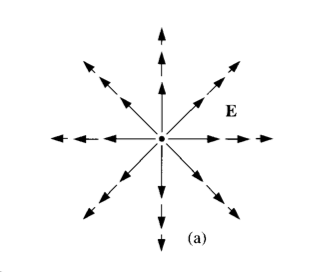
\includegraphics[width=0.99\textwidth]{./images/schematics/electric_field_pos_point_charge.png}\\
   \end{center}
  \end{column}
  \begin{column}{0.50\textwidth}
     The electric field $\vec{E}(\vec{r})$ at a point $\vec{r}$ is given by:
      \begin{equation*}
        \vec{E}(\vec{r}) = \frac{1}{4\pi\epsilon_0} \frac{q}{r^2} \hat{r}
      \end{equation*}
     To visualise the field, we can draw field vectors at various points.\\
     \vspace{0.1cm}
     The field gets smaller away from the charge, so the vectors get shorter.\\
  \end{column}
\end{columns}

\end{frame}

%
%
%

\begin{frame}{Visualising the electric field}

It is impractical to visualise the field as shown before.\\
There is a better way: Connect the arrows! This forms {\em field lines}.\\

\begin{itemize}
\item
  Using field lines we can still visualise the field direction.
\item
  How about the strength (previously represented by the vector size)?
  \begin{itemize}
     \item The field strength is now indicated by the {\bf density} of the field lines.
  \end{itemize}
\end{itemize}

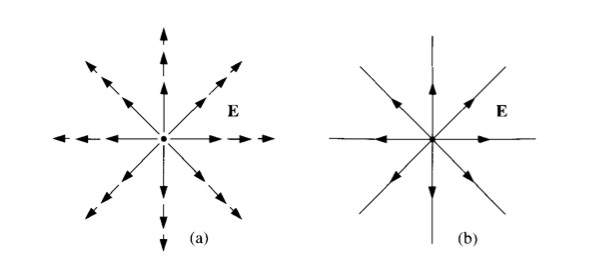
\includegraphics[width=0.95\textwidth]{./images/schematics/electric_field_and_field_lines_pos_point_charge.png}\\

\end{frame}


%
%
%

\begin{frame}{Visualising the electric field}

The electric field $\vec{E}(\vec{r})$ at a point $\vec{r}$, for the simple configuration
we are studying, is given by:
\begin{equation*}
   \vec{E}(\vec{r}) = \frac{1}{4\pi\epsilon_0} \frac{q}{r^2} \hat{r}
\end{equation*}

\vspace{0.2cm}

Obviously, the direction of the field (and thus the {\em flow} of field lines) depends
on the sign of charge q:\\

\vspace{0.2cm}

\begin{center}
  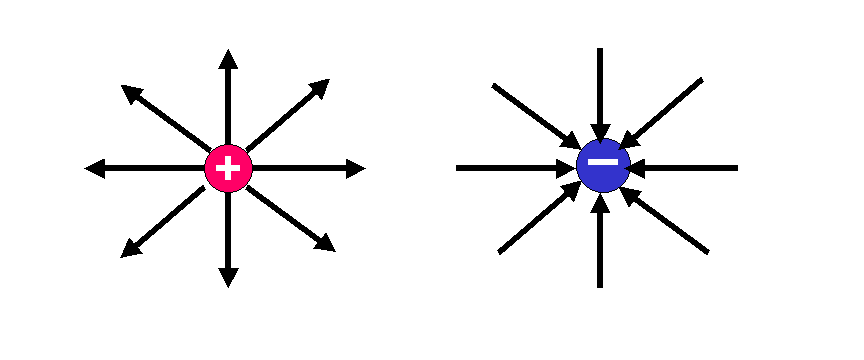
\includegraphics[width=0.98\textwidth]{./images/schematics/electric_field_lines_pos_and_neg_point_charges.png}\\
\end{center}

\end{frame}


%
%
%

\begin{frame}{Electric field lines / A useful analogy}

\begin{columns}
  \begin{column}{0.30\textwidth}
   \begin{center}
     Think of the electric field as the velocity field of air.
     Then the field lines represent the {\em flow} of air.\\
     \vspace{0.5cm}
     Positive charges behave like\\ {\em hair dryers}:\\
     They blow out air.\\
     \vspace{0.3cm}
     Negative charges behave like\\ {\em vacuum cleaners}: \\
     They suck in air.
   \end{center}
  \end{column}
  \begin{column}{0.70\textwidth}
   \begin{center}
    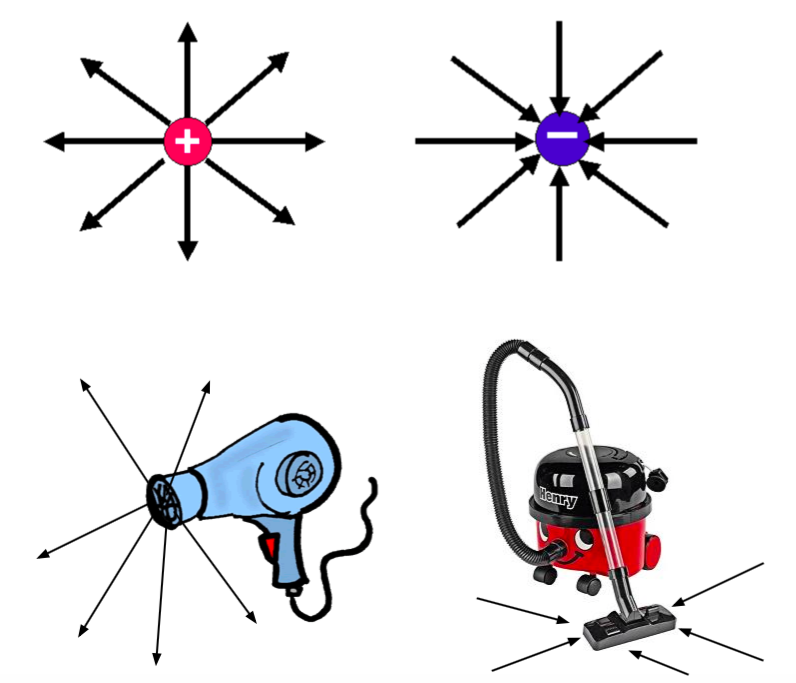
\includegraphics[width=0.98\textwidth]{./images/schematics/electric_field_lines_analogy.png}\\
   \end{center}
  \end{column}
\end{columns}

\end{frame}


%
% Field lines example
%

\begin{frame}{Electric field lines: 2 equal charges}

\begin{center}
 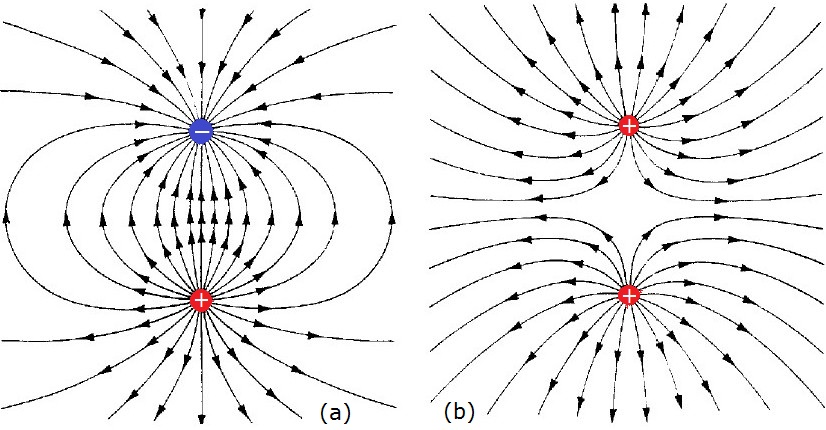
\includegraphics[width=0.90\textwidth]{./images/schematics/electric_field_lines_2_equal_charges_pp_and_np.jpg}
\end{center}

{\small
Field lines start from positive charges and end up in negative charges.\\
The force is tangential to the field lines.
}

\end{frame}

%
% Field lines example
%

\begin{frame}{Electric field lines: 2 unequal charges}

\begin{center}
 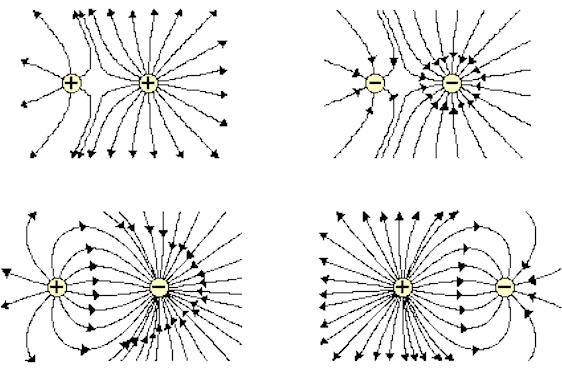
\includegraphics[width=0.75\textwidth]{./images/schematics/electric_field_lines_2_unequal_charges.png}
\end{center}

{\small
Question: Do you understand which of the two charges in each pair is the largest?
}

\end{frame}

%
% Quiz
%

{
\problemslide

\begin{frame}{Quiz}

\begin{blockexmplque}{Question}
  Can electric field lines cross?\\
   \vspace{0.3cm}
   \begin{center}
     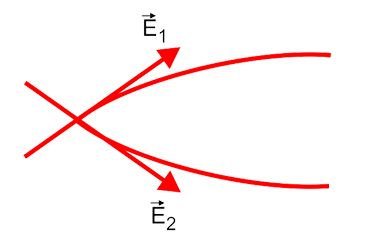
\includegraphics[width=0.45\textwidth]{./images/problems/lect1_impossible_crossing_field_lines.png}\\
   \end{center}
\end{blockexmplque}

\begin{blockexmplans}{Answer}
\noindent
%\scalebox{1}[-1]{
\reflectbox{
 \rotatebox[origin=c]{180}{
   \noindent
   \begin{minipage}[t]{\linewidth}
     Of course not! That would mean that there are points that have two different electric field directions!
   \end{minipage}%
 }
}
\end{blockexmplans}

\end{frame}

} % Quiz


%
% Quiz
%

{
\problemslide

\begin{frame}{Quiz}

\begin{blockexmplque}{Question}
   Now that you understand the basics, can you draw the electric field map for the following configuration
   (light red: negative charges, light blue: positive charges, amount of charge proportional to the circle area)?
   \vspace{0.3cm}
   \begin{center}
     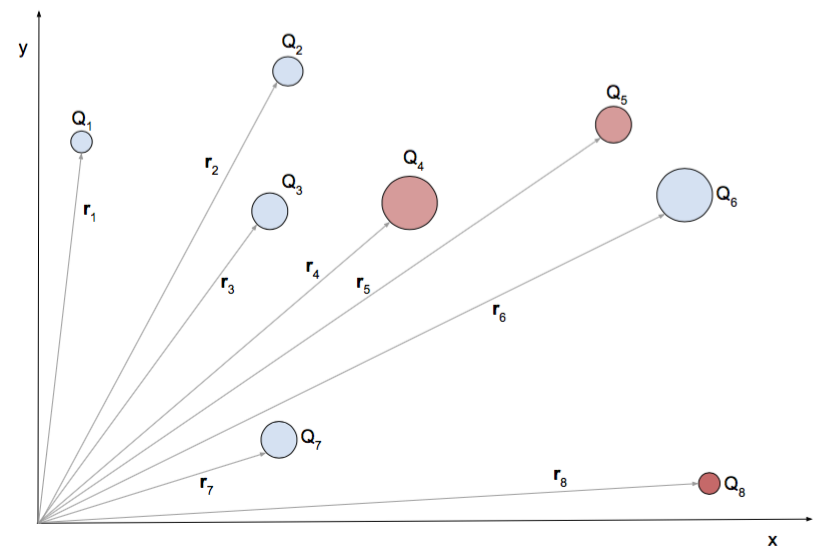
\includegraphics[width=0.45\textwidth]{./images/problems/lect01_n_charges.png}\\
   \end{center}
\end{blockexmplque}

\begin{blockexmplans}{Answer}
\noindent
%\scalebox{1}[-1]{
\reflectbox{
 \rotatebox[origin=c]{180}{
   \noindent
   \begin{minipage}[t]{\linewidth}
     That's what computers are for!
   \end{minipage}%
 }
}
\end{blockexmplans}

\end{frame}

} % Quiz


%
% Programming
%

{
\programmingslide

%
%
%

\begin{frame}{PHYS201 scientific programming task for Lecture \thislecture}

{\small

Write a program that:
\begin{itemize}
{\scriptsize
  \item {\bf Can read an arbitrary distribution of N discrete charges (in 2-D)},\\
        e.g. by accepting as input a text file with N rows, where the $i^{th}$
        row contains the coordinates $x_i$, $y_i$ in m, and the charge $q_i$ in C.
  \item {\bf Allows you to visualise the input charge distribution},\\
        e.g using appropriately-positioned circles whose color or size represents amount of charge.
  \item {\bf Allows you to visualise the electric field lines}
        in the vicinity of the charge distrubution.\\
}
\end{itemize}

\vspace{0.2cm}
Test you program, reproducing some of the simpler field maps shown before.\\

\vspace{0.2cm}
Document your program, upload it to a GitHub repository, and send me a link!\\

\vspace{0.2cm}
Upload images of the most interesting field map you are able to generate!\\

%\vspace{0.2cm}
%You can use any external Python module that helps you do the job!\\
%\begin{itemize}
%  \item {\tt \color{red}matplotlib.pyplot} seems like a suitable tool allowing you to draw vector fields. Google it!
%\end{itemize}

}

\end{frame}


} % programming



%
%
%

\begin{frame}{Electric field due to a continuous charge distribution}

As we saw earlier, the force due to a continuous distribution of charge (distributed in a volume $\tau$) is:
\begin{equation*}
   \vec{F}_{Q} = \frac{Q}{4\pi\epsilon_0} \int_{\tau}
      d\tau^{\prime} \frac{\rho({\pvec{r}'})}{|\vec{r}-\pvec{r}'|^{3}} (\vec{r}-\pvec{r}')
\end{equation*}

Therefore, the electric field in position $\vec{r}$ is:
\begin{equation*}
   \vec{E}(\vec{r}) = \frac{\vec{F}_{Q}}{Q} = \frac{1}{4\pi\epsilon_0} \int_{\tau}
      d\tau^{\prime} \frac{\rho({\pvec{r}'})}{|\vec{r}-\pvec{r}'|^{3}} (\vec{r}-\pvec{r}')
\end{equation*}

The above, is one of the most general results we obtained. In principle, it's all we need to know!
It gives us the electric field $\vec{E}$, and thus the electric force on any charge,
due to an arbitrary distribution of charge.\\

\vspace{0.2cm}
However, the integral involved is very difficult to evaluate.
Much of what follows is about how to compute $\vec{E}$ by {\em avoiding} that complex integration.

\end{frame}



% ------------------------------------------------------------------------------
% ------------------------------------------------------------------------------

%
% Main points to remember
%

\renewcommand{\lecturesummarytitle}{Main points to remember }
\renewcommand{\summarizedlecture}{1 }

%
%
%

\begin{frame}{Lecture \summarizedlecture - \lecturesummarytitle}

\begin{itemize}
{\small
\item {\bf Electric charge}
  \begin{itemize}
  {\small
    \item The source of electric phenomena
    \item An intrinsic property of matter
    \item Comes in two varieties (positive and negative)
    \item An algebraic quantity (+q + (-q) = 0)
    \item It is quantised
    \item It is conserved (globally and locally)
    \item SI unit: Coulomb (C) [= 1 A $\cdot$ 1 s]
  }
  \end{itemize}

\vspace{0.2cm}

\item {\bf Coulomb's law}
  \begin{itemize}
  {\small
     \item Describes the force between two point charges
     \item The force $\vec{F}_{12}$ exerted on test charge 1 by charge 2 is:
     \begin{equation*}
       \vec{F}_{12} = \frac{1}{4\pi\epsilon_0} \frac{q_1 q_2}{|\vec{r}_{1}-\vec{r}_{2}|^{2}} \hat{r}_{12}
       \;\;\;
       or
       \;\;\;
       \vec{F}_{12} = \frac{1}{4\pi\epsilon_0} \frac{q_1 q_2}{|\vec{r}_{1}-\vec{r}_{2}|^{3}} (\vec{r}_{1}-\vec{r}_{2})
     \end{equation*}
  }
  \end{itemize}

}
\end{itemize}

\end{frame}


%
%
%

\begin{frame}{Lecture \summarizedlecture - \lecturesummarytitle (cont'd)}

\begin{itemize}
{\small

\item {\bf Superposition principle}
  \begin{itemize}
  {\small
     \item Allows the calculation of the total force on a charge Q
           from an array of other charges $q_1$, $q_2$, ..., $q_n$
      \begin{equation*}
       \vec{F}_{Q} = \sum_{i=1}^{n} \frac{1}{4\pi\epsilon_0}
          \frac{Q q_i}{|\vec{r}_{Q}-\vec{r}_{q_{i}}|^{3}} (\vec{r}_{Q}-\vec{r}_{q_{i}})
       \end{equation*}
     \item Total force is the vector sum of forces.
     \item Not a logical necessity: An experimental fact!
  }
  \end{itemize}

\vspace{0.2cm}

\item {\bf Continuous distributions of charge}
  \begin{itemize}
  {\small
    \item Made the leap from discrete to continuous charge distributions described by a charge density
    \item Reformulated Coulomb's law for continuous charge distributions
     \begin{equation*}
        \vec{F}_{Q} = \frac{Q}{4\pi\epsilon_0} \int_{\tau}
           d\tau^{\prime} \frac{\rho({\pvec{r}'})}{|\vec{r}-\pvec{r}'|^{3}} (\vec{r}-\pvec{r}')
     \end{equation*}
  }
  \end{itemize}

}
\end{itemize}

\end{frame}

%
%
%

\begin{frame}{Lecture \summarizedlecture - \lecturesummarytitle (cont'd)}

\begin{itemize}
{\small

\item {\bf Electric field}
  \begin{itemize}
  {\small
     \item A more fundamental way to think about electric forces in terms of a field that permeates space.
     \item Defined the electric field $\vec{E}$
           as the force exerted on a test charge Q, placed in position $\vec{r}$, per unit charge.
      \begin{equation*}
        \vec{E}(\vec{r}) = \frac{\vec{F}_Q(\vec{r})}{Q}
      \end{equation*}
  }
  \end{itemize}

\item {\bf Visualizing the electric field - field lines}
  \begin{itemize}
  {\small
     \item Field direction indicated by the direction of field lines
     \item Field strength indicated by the density of field lines
     \item Force tangential to field lines
     \item Field lines start from positive charges and end on negative ones:
           Positive charges are "sources", negative charges are "sinks"
     \item Field lines can not cross
  }
  \end{itemize}
}
\end{itemize}

\end{frame}


%
% At the next lecture
%

\begin{frame}{At the next lecture (Lecture \nextlecture)}

  \begin{itemize}
  {\small
  \item {\bf Electric flux}
    \begin{itemize}
    {\scriptsize
       \item The "flow" of an electric field through a surface.
    }
    \end{itemize}

  \item {\bf Gauss' law}
    \begin{itemize}
    {\scriptsize
       \item Relates the flux through a closed surface with the net charge contained in it.
       \item Our first Maxwell equation! Will study both its `differential' and `integral' forms.
    }
    \end{itemize}
  }
  \end{itemize}

\end{frame}
